%!TEX program = pdflatex
% Mathematics article -- amsart, the neutral class of the subject. Drafting
% here and converting on acceptance costs nothing, because a journal class
% changes the front matter and the page layout and leaves the body alone.
\documentclass[11pt,reqno]{amsart}

\usepackage[margin=1in]{geometry}

% amsart already loads amsmath, amsthm and amsfonts.
\usepackage{amssymb,mathtools}
\usepackage{graphicx}
\usepackage{bm}
\usepackage{xcolor}
\usepackage{cite}
\usepackage{hyperref}
\hypersetup{colorlinks=true,
            linkcolor=blue!55!black,
            citecolor=blue!55!black,
            urlcolor=blue!55!black}
\usepackage[capitalize,nameinlink]{cleveref}

\graphicspath{{figures/}}

\theoremstyle{plain}
\newtheorem{theorem}{Theorem}[section]
\newtheorem{lemma}[theorem]{Lemma}
\newtheorem{proposition}[theorem]{Proposition}
\newtheorem{corollary}[theorem]{Corollary}
\newtheorem{conjecture}[theorem]{Conjecture}

\theoremstyle{definition}
\newtheorem{definition}[theorem]{Definition}
\newtheorem{example}[theorem]{Example}

\theoremstyle{remark}
\newtheorem{remark}[theorem]{Remark}

\numberwithin{equation}{section}

\title[Nilpotency and Loewy length of the kaleidoscope algebra]
{Nilpotency threshold and Loewy length of the kaleidoscope
Yang--Baxter algebra}

\author{Zhiyuan Yao}
\address{Lanzhou Center for Theoretical Physics, \newline
  Key Laboratory of Theoretical Physics of Gansu Province, \newline
  Key Laboratory of Quantum Theory and Applications of MoE, \newline
  Gansu Provincial Research Center for Basic Disciplines of Quantum Physics,
  \newline Lanzhou University, Lanzhou 730000, China}
\email{yaozy@lzu.edu.cn}

\date{\today}

\subjclass[2020]{Primary 16N40, 81R12; Secondary 16S35, 82B23}
\keywords{Kaleidoscope Yang--Baxter equation, quantum torus, nilpotent ideal,
Jacobson radical, Loewy length, Chebyshev polynomial, Bethe ansatz}

\begin{document}

\begin{abstract}
The consistency condition of the coordinate Bethe ansatz on a fan of
$\delta$-function mirrors is a single matrix identity, and it generates a
finite-dimensional algebra spanned by the words in two matrices: a clock
matrix $T$ of order $N$ and a matrix $\Lambda$ of square zero built from the
quantum torus at the $N$th root of unity, both depending on a spectral
parameter $u$. Whether every word in which at least $N/2$ powers of $T$
separate consecutive copies of $\Lambda$ vanishes was left open, with
verification reported only through $N=10$. We prove it for every even
$N=2n\ge4$, every $u$ with $u^N\ne1$ and every tuple of integer exponents. The
mechanism is a flag of subspaces obtained by interpolating separately on the
even and the odd values of $u\omega^{j}+u^{-1}\omega^{-j}$: the operator
$t+t^{-1}$ preserves this flag, every operator $s(t^{k}-t^{-k})$ lowers it by
one step, and a Chebyshev factorization makes the second statement uniform in
the integer $k$. The threshold is sharp. The word with $n-1$ separating
factors, all equal to $T$, has rank two at every admissible $u$, has poles
exactly at $u^{N}=1$ and vanishes nowhere else. Consequently the two-sided
ideal $J$ generated by $\Lambda$ satisfies $J^{n+1}=0$ and $J^{n}\ne0$ and is
the Jacobson radical, so the algebra has $n+1$ nonzero Loewy layers and Loewy
length $N/2+1$, one more than the value proposed with the conjecture, which is
instead the largest exponent with $J^{n}\ne0$. Five properties of the data
carry the whole argument; taken as axioms over an arbitrary field they give
the same threshold, the same sharpness and the same radical, and for each
axiom there is an explicit datum over $\mathbb{Q}$ that satisfies the other
four and violates a conclusion the deleted axiom supports.
\end{abstract}

\maketitle

\section{Introduction}
\label{sec:intro}

A quantum particle in the plane scattering off a fan of $\delta$-function
mirrors through the origin is one of the few two-dimensional problems that a
coordinate Bethe ansatz solves exactly. When the mirror lines carry the
dihedral group of a regular $N$-gon they cut the plane into $2N$ wedges, and
inside each wedge the eigenfunction is a finite superposition of plane waves;
the mirrors relate the amplitudes of neighbouring wedges. These are Gaudin's
generalized kaleidoscopes \cite[Ch.~5]{Gaudin_Book}, named for the mirror
arrangements of classical geometry \cite{Coxeter_Bookig}, and the reflection
groups that classify them are the finite reflection groups
\cite{Humphreys_Book}. The construction descends from the one-dimensional
Bethe ansatz \cite{Bethe_1931zt,Lieb_1963ea,Lieb_1963ea-1,Yang_1967se,Gaudin_1967us,Yang_1966od,Batchelor_2007tb},
and it has been revived by the asymmetric Bethe ansatz of Jackson, Perrin,
Astrakharchik and Olshanii \cite{Jackson_2024ab,Olshanii_2025es}, which
restricts a kaleidoscope solution to the sector odd under the generating
mirrors of a reflection subgroup \cite{Tumarkin_2005rs} and thereby solves
models, such as the mass-imbalanced pair in a hard-wall trap
\cite{Liu_2019mi}, that appear to violate the classical integrability
conditions.

Qiu, Guan and Yu \cite{Qiu_2026ky} showed that the consistency of the ansatz
on the whole fan --- the requirement that an amplitude transported once around
the full circuit of mirrors return to itself --- is one matrix identity, which
they call the kaleidoscope Yang--Baxter equation. Fix an even integer
$N=2n\ge4$ and let $\omega=e^{2\pi\mathrm{i}/N}$. On the standard basis
$e_{0},\dots,e_{N-1}$ of $\mathbb{C}^{N}$, let $t$ be the cyclic shift
$te_{j}=e_{j-1\bmod N}$ and let $d$ be the clock matrix $de_{j}=\omega^{j}e_{j}$,
so that $t^{N}=d^{N}=I$ and $td=\omega\,dt$: the two generate the quantum
torus at the root of unity $\omega$, an algebra that appears as a subalgebra in
the theory of quantum groups \cite{Levendorskii_1991ao} and that carries the
magnetic translations of the quantum Hall effect
\cite{Bellissard_1994tn} and the Fourier modes of noncommutative field theory
\cite{Douglas_2001nf}. The spectral parameter is a complex number
$u=e^{\mathrm{i}\theta}$ recording the incidence angle, and the two matrices
that carry the scattering are
\begin{equation}
  T=\begin{pmatrix}t&0\\0&t^{-1}\end{pmatrix},
  \qquad
  \Lambda=\begin{pmatrix}s&s\\-s&-s\end{pmatrix},
  \qquad
  s=(ud-u^{-1}d^{-1})^{-1},
  \label{eq:intro-generators}
\end{equation}
acting on $\mathbb{C}^{2N}$; here $T$ transports an amplitude past one mirror
and $\Lambda$ carries the strength of the $\delta$-interaction, and the
diagonal matrix $s$ is defined wherever $u^{N}\ne1$. The kaleidoscope
Yang--Baxter equation is the statement that
$[T(I+z\Lambda)]^{N}=I$ for every $z$, and expanding it in $z$ yields
$T^{N}=I$, $\Lambda^{2}=0$ and $(T\Lambda)^{N}=0$.

A fourth statement was left as a conjecture \cite{Qiu_2026ky}: that every word
alternating powers of $T$ with copies of $\Lambda$ dies once enough powers of
$T$ intervene,
\begin{equation}
  \Lambda T^{k_{1}}\Lambda T^{k_{2}}\cdots\Lambda T^{k_{M}}\Lambda=0
  \qquad\text{whenever } M\ge \tfrac{N}{2},
  \label{eq:intro-conjecture}
\end{equation}
for arbitrary integers $k_{1},\dots,k_{M}$. Its authors report that they could
not prove it and verified it only for $N\le10$. The obstacle is not the
identity $\Lambda^{2}=0$, which handles two adjacent copies of $\Lambda$ and
nothing more: each intervening power of $T$ moves the image of the next
$\Lambda$, the exponents are unrestricted integers, and no finite check
reaches every $N$. On the strength of the conjecture the same work describes
the algebra generated by $T$ and $\Lambda$ as splitting into a semisimple part
spanned by the powers of $T$ and a nilpotent ideal generated by $\Lambda$, and
assigns it Loewy length $N/2$.

We prove \cref{eq:intro-conjecture}, prove that its threshold cannot be
lowered, and settle the structural statement that rests on it. Writing
$\mathcal{U}_{N}=\{u\in\mathbb{C}^{\times}:u^{N}\ne1\}$ for the set of
spectral parameters at which $s$ is defined, and $\mathcal{A}$ for the unital
algebra generated by $T$ and $\Lambda$ inside $M_{2N}(\mathbb{C})$, the three
statements are the following.

\begin{theorem}[Threshold and sharpness]
\label{thm:intro-main}
Let $N=2n\ge4$ be even and let $u\in\mathcal{U}_{N}$. Then
\begin{equation*}
  \Lambda T^{k_{1}}\Lambda\cdots\Lambda T^{k_{M}}\Lambda=0
  \qquad\text{for every } M\ge n \text{ and every }
  (k_{1},\dots,k_{M})\in\mathbb{Z}^{M}.
\end{equation*}
At $M=n-1$ the word with $k_{1}=\dots=k_{n-1}=1$ has rank two for every
$u\in\mathcal{U}_{N}$. As a matrix of rational functions of $u$ it has poles
exactly at the $N$th roots of unity, and there is no $u\in\mathcal{U}_{N}$ at
which it vanishes.
\end{theorem}

\begin{theorem}[Radical and Loewy length]
\label{thm:intro-radical}
Let $J=\mathcal{A}\Lambda\mathcal{A}$. Then $J=\operatorname{rad}\mathcal{A}$,
$J^{n+1}=0$ and $J^{n}\ne0$, every inclusion in
$\mathcal{A}\supsetneq J\supsetneq\dots\supsetneq J^{n}\supsetneq J^{n+1}=0$
is strict, and the Loewy length of $\mathcal{A}$ is $n+1=N/2+1$.
\end{theorem}

The value $N/2$ proposed with the conjecture is therefore the largest exponent
$r$ with $J^{r}\ne0$, and not the number of Loewy layers; the two differ by
one, and \cref{thm:intro-radical} fixes which is which.

The kaleidoscope condition sits beside, rather than inside, the two familiar
consistency relations of integrable scattering. The Yang--Baxter equation
equates the two orders in which three components may scatter pairwise, and the
reflection equation of Cherednik \cite{Cherednik_1984fp} and Sklyanin
\cite{Sklyanin_1988bc} adds a boundary; the kaleidoscope condition instead
closes a circuit of $2N$ wedges, and the algebra it generates is nilpotent
above its semisimple part rather than semisimple. A different route to
delta-interactions with reflection symmetry runs through degenerate double
affine Hecke algebras and Dunkl-type operators \cite{Emsiz_2006pi}; it yields
the Bethe ansatz equations and eigenfunctions rather than a finite matrix
algebra, and does not reach the question settled here.

The proof of \cref{thm:intro-main} occupies
\cref{sec:algebra,sec:flag,sec:nilpotency,sec:sharpness} and uses one
mechanism. A similarity that is independent of every exponent turns the
$2N\times2N$ word into a single $N\times N$ word in the quantum torus, built
from the operators $A_{k}=s(t^{k}-t^{-k})$. On $\mathbb{C}^{N}$ we construct a
flag $0=K_{0}\subset K_{1}\subset\dots\subset K_{n}=\mathbb{C}^{N}$ whose $r$th
member consists of the vectors interpolated, separately on the even and the odd
indices $j$, by polynomials of degree less than $r$ in
$y_{j}=u\omega^{j}+u^{-1}\omega^{-j}$. The operator $t+t^{-1}$ preserves each
$K_{r}$ and $A_{1}$ maps $K_{r}$ into $K_{r-1}$; and because
$t^{k}-t^{-k}=(t-t^{-1})q_{k}(t+t^{-1})$ for an integer Chebyshev polynomial
$q_{k}$, so does $A_{k}$, for every integer $k$ at once. A word with $n$ such
factors therefore carries $\mathbb{C}^{N}=K_{n}$ into $K_{0}=0$, and the
degree lowering is exact enough that one factor fewer leaves a rank-two
matrix.

The mechanism uses five properties of the pair $(t,s)$ and the flag, and
nothing else. \Cref{sec:axioms} takes those five as axioms over an arbitrary
field, proves the threshold, the sharpness and the radical statement from them,
and shows that each axiom is indispensable by exhibiting, for each one, an
explicit datum over $\mathbb{Q}$ that satisfies the other four and breaks a
conclusion that axiom supports. \Cref{sec:verification} reports exact
computations run against the original definitions as a check on the
conventions.

\section{The algebra and its scalar reduction}
\label{sec:algebra}

Throughout, $N=2n\ge4$ is even, $\omega=e^{2\pi\mathrm{i}/N}$ is a primitive
$N$th root of unity, $V=\mathbb{C}^{N}$ carries the shift and clock matrices
\begin{equation}
  te_{j}=e_{j-1\bmod N},
  \qquad
  de_{j}=\omega^{j}e_{j}
  \qquad (j\in\mathbb{Z}/N\mathbb{Z}),
  \label{eq:clock-shift}
\end{equation}
and $T$, $\Lambda$ and $s$ are as in \cref{eq:intro-generators}. Reading
\cref{eq:clock-shift} on components, $t$ moves the entries of a vector one
place down the cycle and $d$ multiplies the $j$th entry by $\omega^{j}$; the
two therefore commute up to the fixed phase $\omega$.

The matrix $s$ is diagonal with entries
\begin{equation}
  s_{j}=\bigl(u\omega^{j}-u^{-1}\omega^{-j}\bigr)^{-1},
  \label{eq:sj}
\end{equation}
so $s$ fails to exist exactly where some entry of $ud-u^{-1}d^{-1}$ vanishes.

\begin{lemma}[Admissible domain]
\label{lem:domain}
The matrix $s$ is defined and invertible precisely for
$u\in\mathcal{U}_{N}=\{u\in\mathbb{C}^{\times}:u^{N}\ne1\}$.
\end{lemma}

\begin{proof}
The $j$th entry of $ud-u^{-1}d^{-1}$ vanishes if and only if
$u^{2}\omega^{2j}=1$. Raising that equation to the power $n$ and using
$\omega^{N}=1$ gives $u^{N}=1$. Conversely, if $u^{N}=1$ then $u^{2}$ is an
$n$th root of unity, hence equals $\omega^{-2j}$ for some $j$ because
$\omega^{2}$ has order $n$. Where every entry is nonzero, $s$ is a diagonal
matrix with nonzero entries.
\end{proof}

Every statement below is made for $u\in\mathcal{U}_{N}$, and $T^{N}=I$ lets any
integer exponent on $T$ be reduced modulo $N$ without changing a word.

The block structure of $T$ and $\Lambda$ can be removed once and for all.

\begin{lemma}[Scalar reduction]
\label{lem:reduction}
Put
\begin{equation}
  S=\begin{pmatrix}I&I\\-I&0\end{pmatrix},
  \qquad
  S^{-1}=\begin{pmatrix}0&-I\\I&I\end{pmatrix},
  \qquad
  A_{k}=s(t^{k}-t^{-k}).
  \label{eq:similarity-matrix}
\end{equation}
Then for every $k\in\mathbb{Z}$
\begin{equation}
  S^{-1}T^{k}S=
  \begin{pmatrix}t^{-k}&0\\t^{k}-t^{-k}&t^{k}\end{pmatrix},
  \qquad
  S^{-1}\Lambda S=\begin{pmatrix}0&s\\0&0\end{pmatrix},
  \label{eq:similarity}
\end{equation}
and for all $M\ge1$ and $(k_{1},\dots,k_{M})\in\mathbb{Z}^{M}$
\begin{equation}
  S^{-1}\bigl(\Lambda T^{k_{1}}\Lambda\cdots\Lambda T^{k_{M}}\Lambda\bigr)S
  =\begin{pmatrix}0&A_{k_{1}}A_{k_{2}}\cdots A_{k_{M}}s\\0&0\end{pmatrix}.
  \label{eq:scalar-word}
\end{equation}
\end{lemma}

\begin{proof}
Both identities in \cref{eq:similarity} are a single block multiplication.
In the transformed basis $\Lambda$ has only the upper-right block $s$, so a
product of the two transformed matrices keeps only the upper-right block, and
each factor $S^{-1}T^{k_{i}}S$ contributes its lower-left block $t^{k_{i}}-t^{-k_{i}}$
sandwiched between the two neighbouring copies of $s$. Iterating gives
\cref{eq:scalar-word}.
\end{proof}

\Cref{eq:scalar-word} says that the $2N\times2N$ conjecture is exactly an
$N\times N$ problem: the chained word vanishes if and only if the single
product $A_{k_{1}}\cdots A_{k_{M}}s$ vanishes on $V$. Only the lower-left block
of the transformed $T^{k}$ ever enters, so the diagonal blocks play no part in
what follows.

\begin{remark}
The reference that poses the conjecture prints the lower-right block of the
transformed $T^{p}$ as $t^{-p}$; direct conjugation gives $t^{p}$, as in
\cref{eq:similarity}. Nothing depends on the difference, because only the
lower-left block enters \cref{eq:scalar-word}.
\end{remark}

\section{The parity-polynomial flag}
\label{sec:flag}

Fix $u\in\mathcal{U}_{N}$ and set
\begin{equation*}
  z_{j}=u\omega^{j},
  \qquad
  y_{j}=z_{j}+z_{j}^{-1}
  \qquad (j\in\mathbb{Z}/N\mathbb{Z}).
\end{equation*}
The numbers $y_{j}$ are the interpolation nodes of everything below, and the
parity of $j$ separates them into two classes of $n$ nodes each, because the
shift $t$ exchanges even and odd indices while two shifts return to the class
they started in. In this notation the diagonal entries of $s$ from
\cref{eq:sj} are $s_{j}=(z_{j}-z_{j}^{-1})^{-1}$.

\begin{lemma}[Distinct nodes within each parity]
\label{lem:nodes}
For $u\in\mathcal{U}_{N}$ the $n$ numbers $y_{j}$ with $j$ even are pairwise
distinct, and so are the $n$ numbers $y_{j}$ with $j$ odd.
\end{lemma}

\begin{proof}
For nonzero $a,b$ the equality $a+a^{-1}=b+b^{-1}$ forces $a=b$ or $ab=1$.
Apply this to $a=z_{j}$ and $b=z_{\ell}$ for distinct indices $j,\ell$ of the
same parity. The case $a=b$ gives $\omega^{j-\ell}=1$ with
$0<|j-\ell|<N$, contradicting the primitivity of $\omega$. The case $ab=1$
gives $u^{2}\omega^{j+\ell}=1$; raising it to the power $n$ and using
$\omega^{n}=-1$ yields $u^{N}=(-1)^{j+\ell}=1$, since $j+\ell$ is even, which
contradicts $u\in\mathcal{U}_{N}$.
\end{proof}

Nodes of opposite parity may coincide, and nothing below excludes it: the two
classes are interpolated independently.

\begin{definition}[The flag]
\label{def:flag}
For $0\le r\le n$ let $K_{r}\subseteq V$ be the set of vectors $f$ for which
there exist polynomials $P_{0},P_{1}$ with
$\deg P_{0}<r$ and $\deg P_{1}<r$ such that
\begin{equation*}
  f_{j}=
  \begin{cases}
    P_{0}(y_{j}), & j \text{ even},\\
    P_{1}(y_{j}), & j \text{ odd},
  \end{cases}
\end{equation*}
with $K_{0}=0$.
\end{definition}

A vector of $K_{r}$ is thus described by two independent polynomials, one for
each parity class, of degree less than $r$ in the node variable.

\begin{lemma}[Dimensions]
\label{lem:flag-dim}
$0=K_{0}\subset K_{1}\subset\dots\subset K_{n}=V$ and $\dim K_{r}=2r$.
\end{lemma}

\begin{proof}
By \cref{lem:nodes} the $n$ nodes of a fixed parity are distinct, so on that
class the map sending a polynomial of degree less than $r\le n$ to its values
is injective, and for $r=n$ it is a bijection onto all functions on the class.
Summing the two classes gives $\dim K_{r}=2r$ and $K_{n}=V$.
\end{proof}

Two operators act on this flag:
\begin{equation}
  A=s(t-t^{-1}),
  \qquad
  X=t+t^{-1}.
  \label{eq:AX}
\end{equation}
The first is the $k=1$ member of the family $A_{k}$ of \cref{lem:reduction} and
carries the interaction; the second is the symmetric combination of the two
shifts and carries no $s$. On components, using $(tf)_{j}=f_{j+1}$ and
$(t^{-1}f)_{j}=f_{j-1}$,
\begin{equation}
  (Af)_{j}=\frac{f_{j+1}-f_{j-1}}{z_{j}-z_{j}^{-1}},
  \qquad
  (Xf)_{j}=f_{j+1}+f_{j-1}.
  \label{eq:component-actions}
\end{equation}
Both operators read the two neighbours of the index $j$, which lie in the
parity class opposite to $j$; $A$ takes their difference and divides by the
same quantity that defines $s_{j}$, while $X$ takes their sum.

\begin{lemma}[Propagation and lowering]
\label{lem:lowering}
For $1\le r\le n$,
\begin{equation*}
  XK_{r}\subseteq K_{r},
  \qquad
  AK_{r}\subseteq K_{r-1}.
\end{equation*}
Moreover, if the polynomial representing $f$ on one parity class has degree
$m$ and leading coefficient $c$, then the polynomial representing $Af$ on the
opposite class has degree $m-1$ and leading coefficient
\begin{equation}
  c\,(\omega^{m}-\omega^{-m}),
  \label{eq:leading-coefficient}
\end{equation}
which is nonzero for $1\le m\le n-1$.
\end{lemma}

\begin{proof}
Fix $j$, write $z=z_{j}$, and set $a=y_{j+1}$ and $b=y_{j-1}$. Expanding,
\begin{equation}
  a-b=(\omega-\omega^{-1})(z-z^{-1}),
  \quad
  a+b=(\omega+\omega^{-1})(z+z^{-1}),
  \quad
  ab=(z+z^{-1})^{2}+(\omega-\omega^{-1})^{2}.
  \label{eq:symmetric-data}
\end{equation}
The two elementary symmetric functions of $a$ and $b$ are therefore
polynomials in $y_{j}=z+z^{-1}$ of degrees one and two respectively, while
their difference carries the factor $z-z^{-1}$ that
\cref{eq:component-actions} divides by.

Let $P$ be the polynomial representing $f$ on the parity class of $j\pm1$, so
$f_{j+1}=P(a)$ and $f_{j-1}=P(b)$. The sum $P(a)+P(b)$ is a symmetric
polynomial in $a,b$, hence a polynomial in $a+b$ and $ab$ of weighted degree at
most $\deg P$; by \cref{eq:symmetric-data} it is a polynomial in $y_{j}$ of
degree at most $\deg P$. This proves $XK_{r}\subseteq K_{r}$. Likewise the
divided difference $(P(a)-P(b))/(a-b)$ is symmetric of weighted degree at most
$\deg P-1$, hence a polynomial in $y_{j}$ of degree at most $\deg P-1$; since
\begin{equation}
  (Af)_{j}=\frac{P(a)-P(b)}{z-z^{-1}}
  =(\omega-\omega^{-1})\,\frac{P(a)-P(b)}{a-b},
  \label{eq:divided-difference}
\end{equation}
the operator $A$ drops the degree by at least one, which proves
$AK_{r}\subseteq K_{r-1}$. The middle expression in
\cref{eq:divided-difference} is what $A$ computes, and the right-hand one
exhibits it as a divided difference in the node variable times a constant.

For the leading coefficient take $P(x)=cx^{m}$ plus lower-order terms. Then
$(P(a)-P(b))/(a-b)=c\sum_{i=0}^{m-1}a^{i}b^{m-1-i}$ plus terms of lower degree.
Letting $z\to\infty$ in $a\sim\omega z$, $b\sim\omega^{-1}z$ and $y_{j}\sim z$,
the sum behaves as
$z^{m-1}\omega^{-(m-1)}(\omega^{2m}-1)/(\omega^{2}-1)$, so together with the
prefactor in \cref{eq:divided-difference} the coefficient of $y_{j}^{m-1}$ is
$c(\omega^{m}-\omega^{-m})$. It vanishes only when $\omega^{2m}=1$, that is
when $n$ divides $m$, which is excluded for $1\le m\le n-1$.
\end{proof}

The degree drop is thus not merely an inequality: below the ceiling $n$ it is
exact, and the constant by which the leading coefficient is multiplied never
vanishes. That is what forces the sharpness in \cref{sec:sharpness}, and it
also pins down the Jordan type of $A$.

\begin{corollary}[Jordan type of $A$]
\label{cor:jordan}
For $0\le r\le n$,
\begin{equation}
  \ker A^{r}=K_{r},
  \qquad
  \operatorname{rank}A^{r}=N-2r.
  \label{eq:kernel-rank}
\end{equation}
In particular $A^{n}=0$ and $A$ has exactly two nilpotent Jordan blocks, each
of size $n$.
\end{corollary}

\begin{proof}
By \cref{lem:flag-dim} every $f\in V$ is represented by a unique pair of
polynomials of degree less than $n$, and \cref{lem:lowering} gives
$K_{r}\subseteq\ker A^{r}$. Conversely suppose one of the two polynomials has
degree $m$ with $r\le m\le n-1$. Applying $A$ once transfers it to the opposite
class with degree $m-1$ and a nonzero leading coefficient, by
\cref{eq:leading-coefficient}; the two classes never mix, so after $r$ steps a
polynomial of degree $m-r\ge0$ with nonzero leading coefficient survives and
$A^{r}f\ne0$. Hence $\ker A^{r}=K_{r}$, and \cref{lem:flag-dim} gives the rank.
The kernel dimensions increase by two at each step up to $r=n$, which is the
Jordan type stated.
\end{proof}

\section{Uniform vanishing for arbitrary exponents}
\label{sec:nilpotency}

\Cref{lem:lowering} lowers the flag by the single operator $A=A_{1}$. The step
that makes the argument uniform in the exponents is that every $A_{k}$
factors through $A$.

\begin{lemma}[Integer Chebyshev factorization]
\label{lem:chebyshev}
Define $q_{k}\in\mathbb{Z}[x]$ by
\begin{equation}
  q_{0}=0,
  \qquad
  q_{1}=1,
  \qquad
  q_{k+1}=x\,q_{k}-q_{k-1}\quad(k\ge1),
  \qquad
  q_{-k}=-q_{k}.
  \label{eq:qk}
\end{equation}
Then for every $k\in\mathbb{Z}$
\begin{equation}
  t^{k}-t^{-k}=(t-t^{-1})\,q_{k}(X),
  \qquad\text{hence}\qquad
  A_{k}=A\,q_{k}(X).
  \label{eq:chebyshev}
\end{equation}
\end{lemma}

\begin{proof}
Set $Y_{k}=t^{k}-t^{-k}$. Since $t$ commutes with $t^{-1}$ and hence with $X$,
\begin{equation*}
  XY_{k}=(t+t^{-1})(t^{k}-t^{-k})=Y_{k+1}+Y_{k-1},
\end{equation*}
so $Y_{k+1}=XY_{k}-Y_{k-1}$, which is the recurrence in \cref{eq:qk}. The
cases $k=0$ and $k=1$ of \cref{eq:chebyshev} are immediate, and induction gives
every $k\ge0$; replacing $k$ by $-k$ gives the negative ones, since both sides
change sign. Multiplying on the left by $s$ turns the first identity into the
second.
\end{proof}

The polynomials $q_{k}$ are the Chebyshev polynomials of the second kind in a
normalization that avoids division: $q_{k}(x)=U_{k-1}(x/2)$ for $k\ge1$
\cite{Mason_2002cp}. The recurrence in \cref{eq:qk} has integer
coefficients, so \cref{lem:chebyshev} holds over any commutative ring and in
particular in every characteristic.

\begin{proposition}[Uniform lowering]
\label{prop:uniform-lowering}
For every $k\in\mathbb{Z}$ and every $1\le r\le n$,
\begin{equation}
  A_{k}K_{r}\subseteq K_{r-1}.
  \label{eq:Ak-lowers}
\end{equation}
\end{proposition}

\begin{proof}
By \cref{lem:lowering} the operator $X$ preserves every $K_{r}$, hence so does
any polynomial in $X$; and $A$ lowers the flag by one. Now apply
\cref{eq:chebyshev}.
\end{proof}

\Cref{eq:Ak-lowers} is the whole content of the vanishing half of
\cref{thm:intro-main}: no matter which integer the exponent is --- positive,
zero, negative, or outside any chosen residue system --- the corresponding
operator moves a vector exactly one step down the same flag.

\begin{figure}[t]
  \centering
  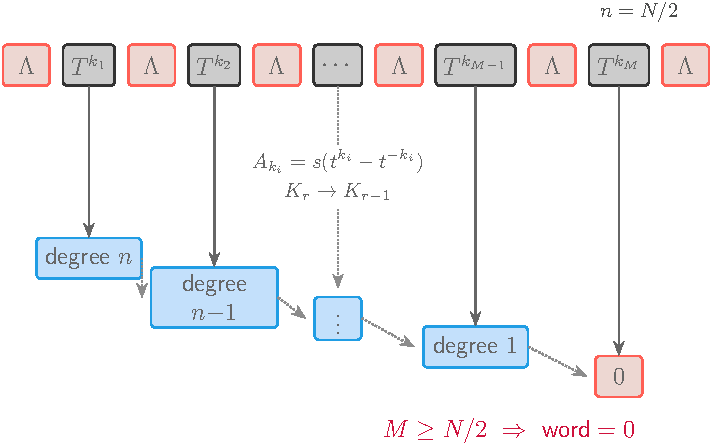
\includegraphics[width=0.80\textwidth]{fig-word-filtration.pdf}
  \caption{How a chained word is forced to zero. Reading the word from the
  right, the invertible factor $s$ maps $\mathbb{C}^{N}$ onto the top member
  $K_{n}$ of the flag, and each intervening power $T^{k_{i}}$ contributes one
  operator $A_{k_{i}}=s(t^{k_{i}}-t^{-k_{i}})$ that carries $K_{r}$ into
  $K_{r-1}$, independently of the integer $k_{i}$. After $n=N/2$ such steps the
  image lies in $K_{0}=0$.}
  \label{fig:filtration}
\end{figure}

\begin{proof}[Proof of the vanishing statement of \cref{thm:intro-main}]
By \cref{lem:reduction} the word $\Lambda T^{k_{1}}\Lambda\cdots\Lambda
T^{k_{M}}\Lambda$ vanishes if and only if $A_{k_{1}}\cdots A_{k_{M}}s$ does.
Read that product from the right, as in \cref{fig:filtration}. Since $s$ is
invertible on $\mathcal{U}_{N}$ by \cref{lem:domain}, $sV=V=K_{n}$ by
\cref{lem:flag-dim}. Each of the $M$ factors $A_{k_{i}}$ then lowers the flag
by one step, by \cref{prop:uniform-lowering}. If $M\ge n$ the image lies in
$K_{0}=0$.
\end{proof}

No ordering, positivity, genericity or congruence condition on the exponent
tuple was used, and $N$ entered only through the length $n$ of the flag.

\section{Sharpness and the pole locus}
\label{sec:sharpness}

One factor fewer does not suffice, and the failure is as large as it can be.

\begin{proposition}[The sharp word]
\label{prop:sharp}
Let $u\in\mathcal{U}_{N}$ and take $M=n-1$ with $k_{1}=\dots=k_{n-1}=1$. Then
the scalar block of the corresponding word is $A^{n-1}s$ and
\begin{equation*}
  \operatorname{rank}\bigl(A^{n-1}s\bigr)=2 .
\end{equation*}
In particular the word is nonzero at every admissible spectral parameter, not
merely at generic ones.
\end{proposition}

\begin{proof}
Define $f\in V$ by $f_{j}=y_{j}^{\,n-1}$ for $j$ even and $f_{j}=0$ for $j$
odd. Applying $A$ repeatedly and using the exact degree drop
\cref{eq:leading-coefficient} at $m=n-1,n-2,\dots,1$,
\begin{equation}
  A^{n-1}f=\Bigl[\prod_{m=1}^{n-1}(\omega^{m}-\omega^{-m})\Bigr]\mathbf{1}_{\epsilon},
  \label{eq:sharp-output}
\end{equation}
where $\mathbf{1}_{\epsilon}$ is the indicator vector of the parity class
reached after $n-1$ transfers. Every factor of the product is nonzero, so
$A^{n-1}f\ne0$; applying $A^{n-1}s$ to $s^{-1}f$ shows $A^{n-1}s\ne0$. The rank
follows from \cref{eq:kernel-rank} at $r=n-1$ together with the invertibility
of $s$.
\end{proof}

\Cref{eq:sharp-output} says that the vector supported on one parity class with
values the top power of the node variable is pushed, in $n-1$ exact steps, to a
nonzero constant vector on the other class.

It remains to locate the singularities of the sharp word as a function of the
spectral parameter, and to check that the points excluded from
$\mathcal{U}_{N}$ are genuine poles rather than removable ones.

\begin{proposition}[Poles and zeros of the sharp word]
\label{prop:poles}
As a matrix of rational functions of $u$, the sharp word $A^{n-1}s$ has poles
exactly at the $N$th roots of unity, each simple in at least one entry, and it
has no zero in $\mathcal{U}_{N}$.
\end{proposition}

\begin{proof}
Absence of zeros in $\mathcal{U}_{N}$ is \cref{prop:sharp}. For the poles, read
$A=s(t-t^{-1})$ in matrix entries: its only nonzero entries are
$A_{j-1,j}=s_{j-1}$ and $A_{j+1,j}=-s_{j+1}$. Fix a column $\ell$ and consider
the entry of $A^{n-1}$ in row $\ell-(n-1)$. A contributing path takes $n-1$
steps of $\pm1$ and must have total displacement $-(n-1)$ modulo $N$; the only
alternative displacement, $-(n-1)+N=n+1$, exceeds the number of steps, so all
steps go the same way and the path is unique. Multiplying by the diagonal $s$
on the right,
\begin{equation}
  \bigl(A^{n-1}s\bigr)_{\ell-(n-1),\,\ell}=\prod_{r=0}^{n-1}s_{\ell-r}.
  \label{eq:unique-path}
\end{equation}
This entry is a product of $n$ consecutive diagonal entries of $s$, with no
competing path to cancel it.

Let $u_{0}^{N}=1$. By the proof of \cref{lem:domain} the entries $s_{j}$ that
blow up at $u_{0}$ are those with $u_{0}^{2}\omega^{2j}=1$, and there are
exactly two of them, at indices differing by $n$. Choose $\ell$ to be one of
the two. The $n$ consecutive indices $\ell,\ell-1,\dots,\ell-(n-1)$ contain
that index and not the other, which is $n$ steps away. The corresponding
denominator $u\omega^{\ell}-u^{-1}\omega^{-\ell}$ has derivative
$2\omega^{\ell}\ne0$ at $u_{0}$, hence a simple zero there, while all the
remaining factors in \cref{eq:unique-path} are finite and nonzero. The entry
therefore has an uncancelled simple pole at $u_{0}$. Since every $s_{j}$ is
finite on $\mathcal{U}_{N}$, there is no pole elsewhere.
\end{proof}

\Cref{prop:sharp,prop:poles} complete \cref{thm:intro-main}: the threshold
$M\ge n$ cannot be replaced by $M\ge n-1$, the counterexample family is
explicit, and its only excluded parameters are exactly the ones at which the
construction is undefined to begin with.

\section{The radical and the Loewy length}
\label{sec:radical}

Let $\mathcal{A}\subseteq M_{2N}(\mathbb{C})$ be the unital algebra generated
by $T$ and $\Lambda$, and let
\begin{equation*}
  J=\mathcal{A}\Lambda\mathcal{A}
\end{equation*}
be the two-sided ideal generated by $\Lambda$, that is, the span of all words
in $T^{\pm1}$ and $\Lambda$ containing at least one $\Lambda$.

\begin{proof}[Proof of \cref{thm:intro-radical}]
Expanding a product of $n+1$ elements of $J$ gives a linear combination of
words each containing at least $n+1$ copies of $\Lambda$. In such a word the
letters between two consecutive copies of $\Lambda$ are powers of $T$, which
combine into a single $T^{k}$ with $k\in\mathbb{Z}$, an empty gap giving
$k=0$. Any $n+1$ consecutive copies of $\Lambda$ therefore form a subword
$\Lambda T^{k_{1}}\Lambda\cdots\Lambda T^{k_{n}}\Lambda$, which vanishes by
\cref{thm:intro-main}, and a word containing a vanishing subword vanishes.
Hence $J^{n+1}=0$. Conversely $(\Lambda T)^{n-1}\Lambda$ is a product of $n$
elements of $J$ and is the sharp word of \cref{prop:sharp}, so
$J^{n}\ne0$.

Because $J$ is a nilpotent two-sided ideal of a finite-dimensional algebra,
$J\subseteq\operatorname{rad}\mathcal{A}$
\cite{Lam_Book}. The quotient $\mathcal{A}/J$ is generated by the
image of $T$, which satisfies $T^{N}=I$, so it is a quotient of
$\mathbb{C}[x]/(x^{N}-1)$. That algebra is semisimple, since $x^{N}-1$ has $N$
distinct roots over $\mathbb{C}$, and a quotient of a semisimple algebra is
semisimple. Hence $\operatorname{rad}(\mathcal{A}/J)=0$, which combined with
$J\subseteq\operatorname{rad}\mathcal{A}$ gives
$\operatorname{rad}\mathcal{A}/J=0$ and therefore
$\operatorname{rad}\mathcal{A}=J$.

For strictness, $I\notin J$ because $J$ is nilpotent, so
$\mathcal{A}\supsetneq J$. If $J^{r}=J^{r+1}$ for some $1\le r\le n$ then
iterating gives $J^{r}=J^{n+1}=0$, contradicting $0\ne J^{n}\subseteq J^{r}$.
Finally, under the standard convention
$\operatorname{LL}(\mathcal{A})=\min\{L\ge1:(\operatorname{rad}\mathcal{A})^{L}=0\}$,
the two displayed facts give $\operatorname{LL}(\mathcal{A})=n+1$.
\end{proof}

The Loewy layers are $\mathcal{A}/J$, $J/J^{2}$, \dots, $J^{n-1}/J^{n}$ and
$J^{n}$, and there are $n+1$ of them, all nonzero. The number $n=N/2$ assigned
to this algebra together with the conjecture \cite{Qiu_2026ky} is the largest
exponent $r$ for which $J^{r}\ne0$; it is one less than the number of layers,
and \cref{thm:intro-radical} is what decides between the two readings, because
it establishes both $J^{n}\ne0$ and $J^{n+1}=0$ rather than only one of them.

\begin{remark}
The decomposition of $\mathcal{A}$ into the span of the powers of $T$ and the
ideal generated by $\Lambda$, proposed with the conjecture, is confirmed by
\cref{thm:intro-radical}: the ideal is precisely the radical, and the quotient
by it is the semisimple algebra generated by the image of $T$.
\end{remark}

\section{A five-axiom family}
\label{sec:axioms}

Nothing in \cref{sec:flag,sec:nilpotency,sec:sharpness,sec:radical} used the
root of unity, the field $\mathbb{C}$, or the interpolation formulas
themselves. Five properties carried the argument, and this section isolates
them, proves the same theorems from them over an arbitrary field, and shows
that none may be dropped.

\begin{definition}[Chebyshev-filtered kaleidoscope datum]
\label{def:datum}
Let $\Bbbk$ be a field, $E$ a finite-dimensional $\Bbbk$-vector space,
$n\ge2$ an integer, and $R,\sigma\in\operatorname{GL}(E)$. Put
\begin{equation*}
  C=R+R^{-1},
  \qquad
  D=\sigma\,(R-R^{-1}),
\end{equation*}
and, on $E\oplus E$,
\begin{equation*}
  \Theta=\begin{pmatrix}R^{-1}&0\\R-R^{-1}&R\end{pmatrix},
  \qquad
  \Xi=\begin{pmatrix}0&\sigma\\0&0\end{pmatrix},
  \qquad
  \mathcal{K}=\Bbbk\langle I,\Theta,\Xi\rangle,
  \qquad
  \mathcal{J}=\mathcal{K}\,\Xi\,\mathcal{K}.
\end{equation*}
A \emph{length-$n$ Chebyshev-filtered kaleidoscope datum} is such a tuple
together with a chain of subspaces $F_{0},\dots,F_{n}$ of $E$ obeying
\begin{itemize}
  \item[(A1)] \emph{exhaustive flag of width two:}
    $0=F_{0}\subset F_{1}\subset\dots\subset F_{n}=E$ and $\dim F_{r}=2r$;
  \item[(A2)] \emph{propagation:} $CF_{r}\subseteq F_{r}$ for $0\le r\le n$;
  \item[(A3)] \emph{lowering:} $DF_{r}\subseteq F_{r-1}$ for $1\le r\le n$;
  \item[(A4)] \emph{survival:} $D^{\,n-1}\ne0$;
  \item[(A5)] \emph{semisimple cyclic carrier:}
    $B=\Bbbk[\Theta,\Theta^{-1}]$ is semisimple.
\end{itemize}
\end{definition}

The operator $C$ is the abstract counterpart of $X=t+t^{-1}$ and $D$ of
$A=s(t-t^{-1})$; the block matrices $\Theta$ and $\Xi$ are what the similarity
of \cref{lem:reduction} turns $T$ and $\Lambda$ into. Invertibility of $R$ and
$\sigma$ is part of the data rather than a sixth axiom: it is what gives
negative powers a meaning and what transports nonvanishing through the
rightmost factor.

Over a field on which equality, linear algebra and polynomial factorization
can be carried out, the five conditions are finite checks: (A1) from the ranks
of the flag bases, (A2) and (A3) by reducing $C$ and $D$ applied to a flag
basis against the target basis, (A4) from $\operatorname{rank}D^{\,n-1}$, and
(A5) --- since $\Theta$ is invertible and hence $B=\Bbbk[\Theta]$ --- from the
absence of a repeated irreducible factor in the minimal polynomial of $\Theta$.
Over an arbitrary field they remain algebraic conditions with no claim of
decidability.

\begin{proposition}[The original model is a datum]
\label{prop:embedding}
Let $N=2n\ge4$ be even and $u\in\mathcal{U}_{N}$. Take $\Bbbk=\mathbb{C}$,
$E=V=\mathbb{C}^{N}$, $R=t$, $\sigma=s$ and $F_{r}=K_{r}$. Then all five
axioms hold, $C=X$ and $D=A$, and $\Theta=S^{-1}TS$, $\Xi=S^{-1}\Lambda S$, so
$\mathcal{K}$ is similar to $\mathcal{A}$ and $\mathcal{J}$ to $J$.
\end{proposition}

\begin{proof}
The identifications of $C$, $D$, $\Theta$ and $\Xi$ are \cref{eq:AX} and
\cref{eq:similarity}. Axiom (A1) is \cref{lem:flag-dim}, (A2) and (A3) are
\cref{lem:lowering}, and (A4) is \cref{eq:kernel-rank} at $r=n-1$, which gives
$\operatorname{rank}A^{n-1}=2$. For (A5), $t^{N}=I$ gives $\Theta^{N}=I$ by
\cref{eq:similarity}, so the minimal polynomial of $\Theta$ divides $x^{N}-1$,
which is square-free over $\mathbb{C}$.
\end{proof}

The embedding is uniform: it holds at every even $N$ and every admissible $u$
at once, with no genericity condition.

\begin{lemma}[Block powers and the sandwich]
\label{lem:blocks}
With $q_{k}$ as in \cref{eq:qk}, for every $k\in\mathbb{Z}$
\begin{equation*}
  R^{k}-R^{-k}=(R-R^{-1})\,q_{k}(C),
  \qquad
  \Theta^{k}=\begin{pmatrix}R^{-k}&0\\R^{k}-R^{-k}&R^{k}\end{pmatrix},
\end{equation*}
and consequently
\begin{equation}
  \Xi\,\Theta^{k}\,\Xi=\begin{pmatrix}0&D\,q_{k}(C)\,\sigma\\0&0\end{pmatrix}.
  \label{eq:sandwich}
\end{equation}
\end{lemma}

\begin{proof}
The first identity is \cref{lem:chebyshev} with $t$ replaced by $R$; its proof
used only that $R$ commutes with $R^{-1}$, and the recurrence
\cref{eq:qk} has integer coefficients, so it is valid over any field. The
second holds for $k=0,1$ and propagates: multiplying the displayed matrix by
$\Theta$ sends the lower-left block to
$(R^{k}-R^{-k})R^{-1}+R^{k}(R-R^{-1})=R^{k+1}-R^{-(k+1)}$ and the diagonal
blocks to $R^{-(k+1)}$ and $R^{k+1}$. Block inversion gives
$\Theta^{-1}=\bigl(\begin{smallmatrix}R&0\\R^{-1}-R&R^{-1}\end{smallmatrix}\bigr)$,
and the same induction covers $k<0$. Multiplying out
$\Xi\Theta^{k}\Xi$ leaves only the upper-right block, which is
$\sigma(R^{k}-R^{-k})\sigma=Dq_{k}(C)\sigma$.
\end{proof}

\Cref{eq:sandwich} fixes the order of the factors: the lowering operator $D$
stands to the left of the polynomial $q_{k}(C)$, not to its right.

\begin{theorem}[Axiomatic threshold and sharpness]
\label{thm:abstract-main}
Let $(E,R,\sigma,F_{\bullet})$ be a length-$n$ Chebyshev-filtered kaleidoscope
datum. Then
\begin{equation}
  \Xi\,\Theta^{k_{1}}\,\Xi\cdots\Xi\,\Theta^{k_{M}}\,\Xi=0
  \qquad\text{for all } M\ge n,\ (k_{1},\dots,k_{M})\in\mathbb{Z}^{M},
  \label{eq:abstract-vanishing}
\end{equation}
while at $M=n-1$ and $k_{1}=\dots=k_{n-1}=1$ the same word is nonzero. Only
(A1), (A2) and (A3) are used for the vanishing, and (A4) only for the
nonvanishing.
\end{theorem}

\begin{proof}
Iterating \cref{eq:sandwich}, the only possibly nonzero block of the word in
\cref{eq:abstract-vanishing} is the upper-right one,
$D\,q_{k_{1}}(C)\,D\,q_{k_{2}}(C)\cdots D\,q_{k_{M}}(C)\,\sigma$. By (A2) every
polynomial in $C$ preserves every $F_{r}$, so by (A3) each composite
$Dq_{k}(C)$ carries $F_{r}$ into $F_{r-1}$. Since $\sigma$ is invertible,
$\sigma E=E=F_{n}$ by (A1). Reading the product from the right, $M\ge n$
lowering steps land in $F_{0}=0$. For the sharp word $q_{1}=1$, so the
upper-right block is $D^{\,n-1}\sigma$, nonzero by (A4) and the surjectivity of
$\sigma$.
\end{proof}

\begin{theorem}[Radical and layers from the axioms]
\label{thm:abstract-radical}
For every length-$n$ Chebyshev-filtered kaleidoscope datum,
\begin{equation*}
  \mathcal{J}=\operatorname{rad}\mathcal{K},
  \qquad
  \mathcal{J}^{\,n+1}=0,
  \qquad
  \mathcal{J}^{\,n}\ne0,
\end{equation*}
every inclusion in
$\mathcal{K}\supsetneq\mathcal{J}\supsetneq\dots\supsetneq\mathcal{J}^{\,n}\supsetneq
\mathcal{J}^{\,n+1}=0$ is strict, and $\mathcal{K}$ has exactly $n+1$ nonzero
Loewy layers.
\end{theorem}

\begin{proof}
The argument of \cref{thm:intro-radical} applies verbatim with
\cref{thm:abstract-main} in place of \cref{thm:intro-main}: a product of $n+1$
elements of $\mathcal{J}$ expands into words with $n+1$ copies of $\Xi$
separated by powers of $\Theta$, each containing a vanishing subword; and
$(\Xi\Theta)^{n-1}\Xi$ is a nonzero product of $n$ elements of $\mathcal{J}$.
For the radical, $\mathcal{K}/\mathcal{J}$ is generated by the image of
$\Theta$, so the natural map $B\to\mathcal{K}/\mathcal{J}$ is surjective;
axiom (A5) makes $B$ semisimple, hence so is its quotient, and the two
inclusions close as before. Strictness follows from
$\mathcal{J}^{\,n}\ne0$ exactly as in \cref{thm:intro-radical}.
\end{proof}

No formula for the dimension of an individual layer
$\mathcal{J}^{\,r}/\mathcal{J}^{\,r+1}$ is claimed; the axioms fix how many
layers there are and that each is nonzero, not how large each one is.

\subsection*{Every axiom is needed}

Each of the five axioms is now shown to be independent: for each one there is a
finite-dimensional datum over $\mathbb{Q}$ that satisfies the other four and
violates a conclusion the deleted axiom supports. All five constructions are
exact, with no fitted parameter and no genericity assumption.

Two conventions keep the examples small. When base data $R_{0},\sigma_{0}$ on
$E_{0}$ and a base flag $G_{0}\subset\dots\subset G_{n}$ are displayed, the
datum is the doubling $E=E_{0}\oplus E_{0}$, $R=R_{0}\oplus R_{0}$,
$\sigma=\sigma_{0}\oplus\sigma_{0}$ and $F_{r}=G_{r}\oplus G_{r}$, which turns
$\dim G_{r}=r$ into the width $\dim F_{r}=2r$ that (A1) demands. And for any
invertible $R$ the matrix $S$ of \cref{eq:similarity-matrix} conjugates
$\operatorname{diag}(R,R^{-1})$ into $\Theta$, so (A5) holds whenever $R$ is
diagonalizable with a square-free minimal polynomial; in particular it holds
for every diagonal $R_{0}$ with distinct nonzero entries.

\begin{theorem}[Independence]
\label{thm:independence}
For each axiom in $\{\mathrm{(A1)},\dots,\mathrm{(A5)}\}$ there is a
finite-dimensional datum over $\mathbb{Q}$ satisfying the other four and
falsifying a conclusion of
\cref{thm:abstract-main} or \cref{thm:abstract-radical} that the deleted axiom
supports.
\end{theorem}

\begin{proof}
We give one witness for each axiom.

\emph{Deleting} (A1). Let $n=2$, $E_{0}=\mathbb{Q}^{3}$,
\begin{equation*}
  R_{0}=\operatorname{diag}(1,2,3),
  \qquad
  \sigma_{0}=\begin{pmatrix}0&2/3&0\\1&0&0\\0&0&3/8\end{pmatrix},
\end{equation*}
and $G_{0}=0$, $G_{1}=\langle e_{1}\rangle$ and
$G_{2}=\langle e_{1},e_{2}\rangle$, a proper subspace of $E_{0}$. Then
$C_{0}=\operatorname{diag}(2,5/2,10/3)$ and
$D_{0}=\sigma_{0}\operatorname{diag}(0,3/2,8/3)$ has $D_{0}e_{1}=0$,
$D_{0}e_{2}=e_{1}$ and $D_{0}e_{3}=e_{3}$. Axiom (A2) holds because $C_{0}$ is
diagonal, (A3) because $D_{0}G_{1}=0$ and $D_{0}G_{2}\subseteq G_{1}$, (A4)
because $D\ne0$, and (A5) because $R_{0}$ is diagonal with distinct entries.
Only exhaustivity fails, and $D_{0}^{2}e_{3}=e_{3}$, so $D^{2}\sigma\ne0$ and
the threshold word at $M=n=2$ survives.

\emph{Deleting} (A2). Let $n=3$, $E_{0}=\mathbb{Q}^{3}$, $v=e_{2}+e_{3}$,
\begin{equation*}
  R_{0}=\operatorname{diag}(1,2,3),
  \qquad
  \sigma_{0}=\begin{pmatrix}0&2/3&0\\1&-2/3&3/8\\-1&-2/3&3/8\end{pmatrix},
\end{equation*}
and $G_{1}=\langle e_{1}\rangle$, $G_{2}=\langle e_{1},v\rangle$,
$G_{3}=E_{0}$. Then $C_{0}=\operatorname{diag}(2,a,b)$ with $a=5/2$ and
$b=10/3$, and $D_{0}e_{1}=0$, $D_{0}e_{2}=e_{1}-v$, $D_{0}e_{3}=v$. Axioms
(A1), (A3), (A4) and (A5) hold; in particular $D_{0}v=e_{1}$ and
$D_{0}^{2}e_{3}=e_{1}\ne0$. But $C_{0}v=ae_{2}+be_{3}\notin G_{2}$ because
$a\ne b$, so (A2) fails. With $\delta=b-a=5/6$ and $q_{2}(x)=x$, a direct
computation gives
\begin{equation*}
  (D_{0}C_{0})^{3}e_{3}=b\,\delta\,(a\,e_{1}+\delta\,v)\ne0,
\end{equation*}
so the threshold tuple $(2,2,2)$ survives at $M=n=3$. The failure is exactly
the one (A2) forbids: the polynomial $q_{2}(C)$ pushes a vector back up the
flag faster than $D$ pulls it down.

\emph{Deleting} (A3). Let $n=2$, $R_{0}=\operatorname{diag}(2,3)$,
$\sigma_{0}=I_{2}$, $G_{1}=\langle e_{1}\rangle$ and $G_{2}=E_{0}$. Then
$C_{0}=\operatorname{diag}(5/2,10/3)$ and
$D_{0}=\operatorname{diag}(3/2,8/3)$, so (A1), (A2), (A4) and (A5) hold while
$D_{0}G_{1}=G_{1}\not\subseteq G_{0}=0$. Since $D_{0}^{2}\ne0$, the threshold
word at $M=2$ survives.

\emph{Deleting} (A4). Let $n=3$, $E=\mathbb{Q}^{6}$, $R=\sigma=I_{6}$ and
$F_{r}=\langle e_{1},\dots,e_{2r}\rangle$. Then $C=2I$, $D=0$ and
$\Theta=I$, so (A1), (A2), (A3) and (A5) hold while $D^{\,n-1}=0$. Here
$\mathcal{K}=\mathbb{Q}I\oplus\mathbb{Q}\Xi$ and
$\mathcal{J}=\mathbb{Q}\Xi$ with $\mathcal{J}^{2}=0$, so the Loewy length is
$2$ rather than $n+1=4$: without (A4) the layer count of
\cref{thm:abstract-radical} collapses.

\emph{Deleting} (A5). Let $n=2$, put
$\mathcal{N}=\bigl(\begin{smallmatrix}0&1\\0&0\end{smallmatrix}\bigr)$,
\begin{equation*}
  R_{0}=I_{2}+\mathcal{N},
  \qquad
  \sigma_{0}=\tfrac12 I_{2},
\end{equation*}
and $G_{1}=\ker\mathcal{N}=\langle e_{1}\rangle$, $G_{2}=E_{0}$. Since
$\mathcal{N}^{2}=0$ one has $R_{0}^{-1}=I_{2}-\mathcal{N}$, hence $C_{0}=2I$
and $D_{0}=\mathcal{N}$, so (A1)--(A4) hold. The minimal polynomial of
$\Theta$ is $(x-1)^{2}$, so (A5) fails. Write $H=\Theta-I$; on one summand of
the doubling
\begin{equation*}
  H=\begin{pmatrix}-\mathcal{N}&0\\2\mathcal{N}&\mathcal{N}\end{pmatrix},
  \qquad
  \Xi=\begin{pmatrix}0&\tfrac12 I_{2}\\0&0\end{pmatrix},
\end{equation*}
and $H^{2}=\Xi^{2}=H\Xi H=0$. Those three relations close the algebra:
\begin{equation*}
  \mathcal{K}=\operatorname{span}_{\mathbb{Q}}\{I,H,\Xi,H\Xi,\Xi H,\Xi H\Xi\},
  \qquad
  \mathcal{J}=\operatorname{span}_{\mathbb{Q}}\{\Xi,H\Xi,\Xi H,\Xi H\Xi\}.
\end{equation*}
Every spanning matrix of $\mathcal{J}$ has zero lower-left block, whereas the
lower-left block of $H$ is $2\mathcal{N}\ne0$; hence $H\notin\mathcal{J}$. The
class of $H$ in $\mathcal{K}/\mathcal{J}$ is then nonzero with square zero, so
$\operatorname{rad}(\mathcal{K}/\mathcal{J})\ne0$ and
$\mathcal{J}\subsetneq\operatorname{rad}\mathcal{K}$: without (A5) the ideal
generated by $\Xi$ is still nilpotent but is no longer the whole radical. The
doubled datum is two faithful copies of this algebra, so the same
ideal-membership argument applies to it.
\end{proof}

Each witness removes one axiom and keeps the other four, so
\cref{thm:independence} is a statement about necessity and not merely a list of
ways the hypotheses can fail. Read together with \cref{prop:embedding}, it says
that the five conditions are a minimal description of what makes the
kaleidoscope algebra behave as \cref{thm:intro-main,thm:intro-radical} say it
does.

\section{Independent exact checks}
\label{sec:verification}

The results above are proved without computation, and the reader can follow
every step from the page. Exact computations were nevertheless carried out
against the definitions, as a check on the conventions --- the direction of the
shift, the order of the factors in a word, the treatment of negative and zero
exponents, and the behaviour at parameters where nodes of opposite parity
collide. They are reported here because each one is a way the argument could
have been wrong without being visibly wrong.

Reconstructing $t$, $d$, $s$, $T$ and $\Lambda$ over the field with $97$
elements, which contains primitive $4$th, $6$th and $8$th roots of unity, one
can enumerate threshold words exhaustively rather than sample them. For $N=4$
and $N=6$ every admissible spectral parameter in that field was used --- $92$
and $90$ values respectively, the excluded ones being the roots of $u^{N}=1$
--- together with every exponent tuple $(k_{1},\dots,k_{n})$ with
$0\le k_{i}<N$, giving $16$ and $216$ tuples per parameter. For $N=8$ all
$4096$ tuples were used at three admissible parameters, one of them satisfying
$u^{8}=-1$, where the even and odd node sets intersect while each remains
internally distinct, as \cref{lem:nodes} allows. The three families comprise
$33{,}200$ words. Every one vanished, and at every parameter the all-ones word
one step below the threshold was nonzero of rank two.

A separate computation in characteristic zero, over exact algebraic
extensions, constructed the sharp word $A^{n-1}s$ for $N=4,6,8$. In each case
its rank is two, the radical of the common denominator of its entries is
$u^{N}-1$, and its nonzero entries have no common zero in
$\mathbb{C}^{\times}$; these are \cref{prop:sharp,prop:poles} at three sizes,
obtained from the matrix definitions rather than from the interpolation
argument.

For the axiomatic family, the block-power and sandwich identities of
\cref{lem:blocks} were checked to have vanishing residual for every exponent
from $-3$ to $3$ and for mixed tuples of positive, zero and negative exponents,
with a non-diagonal $R$ and a $\sigma$ that does not commute with it. In one
explicit datum over $\mathbb{Q}$ of length $n=2$, all $25$ threshold words with
exponents in $\{-2,\dots,2\}$ vanish while the sharp word has rank two. The
five witnesses of \cref{thm:independence} were rebuilt from the displayed
matrices and each was found to satisfy exactly four of the five axioms; the
three surviving threshold words have ranks $2$, $2$ and $4$, the datum
deleting (A4) has Loewy length $2$, and the datum deleting (A5) has
$\dim\mathcal{K}=6$, $\dim\mathcal{J}=4$, $\dim\mathcal{J}^{2}=1$,
$\mathcal{J}^{3}=0$ and $H\notin\mathcal{J}$.

None of these computations is a premise of any statement above. They rule out
the transcription and convention errors that a purely symbolic argument cannot
rule out about itself, and they agree with it everywhere.

\section{Conclusion}
\label{sec:conclusion}

Words in the kaleidoscope Yang--Baxter algebra die at a threshold set by half
the clock order, and they do so for one reason: the operator
$s(t-t^{-1})$ is a divided difference in the variable
$y_{j}=u\omega^{j}+u^{-1}\omega^{-j}$ and therefore lowers polynomial degree,
$t+t^{-1}$ is a symmetric function of the same two shifts and therefore does
not raise it, and the integer Chebyshev identity
$t^{k}-t^{-k}=(t-t^{-1})q_{k}(t+t^{-1})$ makes every intervening power of $T$
act like the first one. Since the two parity classes carry $n=N/2$ distinct
nodes each, $n$ lowering steps exhaust the flag and every word with $n$
intervening powers vanishes, for every even $N$, every admissible spectral
parameter and every tuple of integer exponents. One step fewer leaves a matrix
of rank two whose poles are exactly the $N$th roots of unity and which
vanishes at no admissible parameter, so the threshold is sharp in the strongest
available sense. The ideal generated by $\Lambda$ is therefore the Jacobson
radical, its $(n+1)$st power vanishes and its $n$th does not, and the algebra
has $n+1=N/2+1$ Loewy layers --- one more than the value that was proposed
with the conjecture, which counts instead the largest nonvanishing radical
power.

The mechanism is not tied to the root of unity or to the complex field. Five
conditions --- an exhaustive flag of width two, a propagating symmetric
operator, a lowering operator, survival of its $(n-1)$st power, and a
semisimple cyclic carrier --- reproduce the threshold, the sharpness and the
radical over an arbitrary field, and each of the five is necessary, as an
explicit rational counterexample for the deletion of each one shows.

What lies immediately beyond is the size rather than the number of the layers:
the axioms fix that there are $n+1$ nonzero Loewy quotients but say nothing
about the dimension of each, and a classification of the data satisfying them
is open. Odd clock order, spectral parameters on the excluded circle, other
representations of the kaleidoscope Yang--Baxter relation, and the
consequences of the filtration for the spectrum of the underlying scattering
problem all lie outside the argument given here. A single admissible exponent
tuple at the threshold with a nonzero word, or a single admissible parameter at
which the all-ones word one step below it vanishes, would refute what is proved
here; none exists.

\section*{Acknowledgments}

Z.\ Y.\ acknowledges support from the Strategic Priority Research Program of the
Chinese Academy of Sciences under Grant No.~XDB1680102. Z.\ Y.\ also
acknowledges support by National Natural Science Foundation of China (Grant
No.~12247101). We also acknowledge Gewu Intelligence Lab for providing the
collaborative research environment in which this project was developed.

OpenAI GPT-5.6 Sol was used substantively in this work: in solving the
problem, including the formulation of arguments and the derivation of
intermediate steps, and in drafting and revising the manuscript. The authors
specified the problem, guided the approach to be taken, checked every argument
and result it produced, and take full responsibility for the content of this
manuscript.

\bibliographystyle{unsrt}
\bibliography{references,unverified}

\end{document}
